% Use class option [extendedabs] to prepare the 1-page extended abstract.
\documentclass[extendedabs]{bmvc2k}
\usepackage[colorlinks = true,
            linkcolor = blue,
            urlcolor  = blue,
            citecolor = blue,
            anchorcolor = blue]{hyperref}
\usepackage{kotex}
% for the fancy \koTeX logo
\usepackage{kotex-logo}
\usepackage{mathtools}  % brings in amsmath, also some improvements
\usepackage{amssymb} % brings in amsfonts, incl \square
% Document starts here
\usepackage{graphicx}
\begin{document}


\title{CLIP and Linearly Mapping pre-report}
\addauthor{
Taehun Kim$^{1}$
}{}{1}

\addinstitution{
$^1$ Department of Computer Science and Engineering, Pusan National University.  
}
 

\maketitle
\noindent

\section{CLIP}
\begin{figure}[t]
\centering
	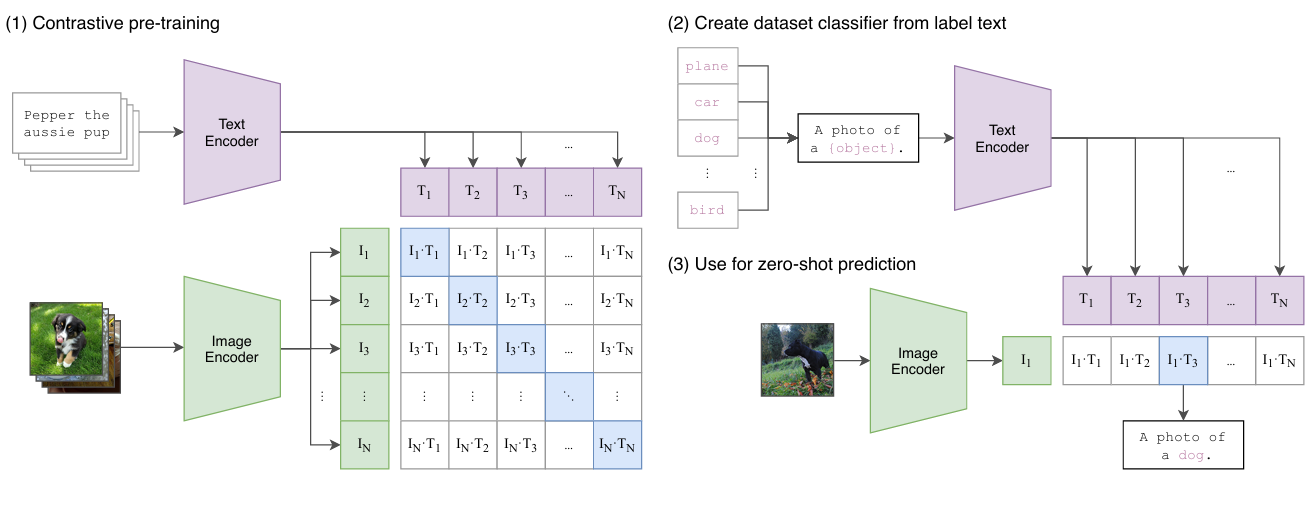
\includegraphics[width=\linewidth]{images/fig1.PNG}
	\caption{
		Summary of the approach. CLIP jointly trains an image encoder and a text encoder to predict the correct pairing of a batch of (image,text) pairs. At test time the trained text-encoder synthesizes a zero-shot classifier by embedding the names or description of the target dataset's class.}
	\vspace{-2mm}
        \label{fig:clipapproach}
\end{figure}
\subsection{Introduction}
We summarize the CLIP paper\cite{clip} in this section. Contrastive Language-Image Pre-Training(CLIP) learns directly from raw text about the image, and is competitive with a full supervised model with few-shot or zero-shot learning. Additionally, zero-shot CLIP models are much more robust than supervised ImageNet model.

Recent NLP models such as GPT-3 learned directly from raw text from the Web and are competitive with a bespoke model, while requiring little or no additional data. This is made possible because of task-agnostic objectives, such as masked language modeling and text-to-text as a standardized input-output interface.

These results suggest that the pretraining method with web-scale text collections exceeds that with crowd-labeled data. However, pre-training on crowd-labeled datasets such as ImageNet remains a standard practice in the field of computer vision. 

The authors create a new dataset of 400 million (image,text) pairs and demonstrate that CLIP is an efficient method of learning from natural language supervision. In the section below, we look at CLIP's approach.
\subsection{Natural Language Supervision}
Core of this approach is learning from supervision contained in natural language. This approach has several strengths. It is much easier to scale than crowd-labeled data. Natural language supervision also has the advantage of connecting representations to language, which enables flexible zero-shot transfer.
\subsection{Creating a Sufficiently Large Dataset}
For training natural language supervision, large quantity of data from the Internet is required. To address this, The authors constructed a new dataset of 400 million (image,text) pairs collected from the variety sources on the Internet. They use 500,000 queries, and include up to 20,000 pairs per query for balancing.
\subsection{Selecting an Efficient Pre-Training Method}
For efficient scaling, the authors use contrastive learning with bag-of-words encoding. This is because Transformer model has more parameters than ResNet-50 image encoder, and is slower than a bag-of-words encoding.

CLIP is trained using a batch of $N$ (image, text) pairs. As shown in Fig \ref{fig:clipapproach}, an image is encoded by an image encoder such as ResNet-50, and a text is encoded by an text encoder such as Transformer. The encoded image and text are projected onto embedding vectors using the image embedding matrix and text embedding matrix, respectively. 

CLIP learns these embedding space by jointly training an image encoder and text encoder to maximize the cosine similarity of the image and text embedding of the $N$ real pairs in the batch while minimizing the cosine similarity of the embedding of the remain incorrect pairings. After that, the loss is computed using cross-entropy loss based on the cosine similarity. $loss_i$ is the cross-entropy loss computed along axis=0, treating the cosine similarity as predictions of image embeddings relative to text embeddings. $loss_t$ is the cross entropy loss computed along axis=1, treating the cosine similarity as prediction of text embeddings relative to image embedding. The final loss is the average of $loss_i$ and $loss_t$. This metric is called \textit{multi-class N-pair loss}:

$$
labels = np.arange(n)
$$
$$
loss_i = \textbf{cross-entropy-loss}(cossim, labels,axis=0)
$$
$$
loss_j = \textbf{cross-entropy-loss}(cossim, labels,axis=1)
$$
$$
loss = (loss_i + loss_t)/2
$$

\begin{figure}[t]
\centering
	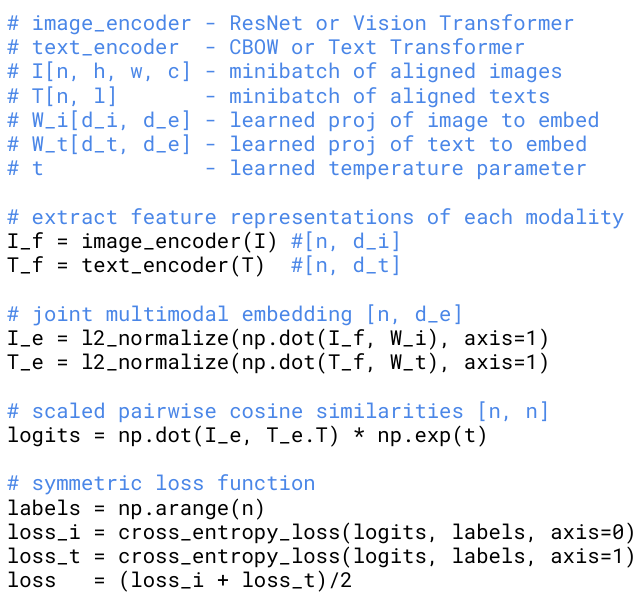
\includegraphics[width=\linewidth]{images/fig2.PNG}
	\caption{
		 pseudocode for the core of an implementation of CLIP.}
	\vspace{-2mm}
        \label{fig:clipcode}
\end{figure}

Due to the large size of the pre-training dataset, over-fitting is not a major concern and the author train CLIP without initializing with pre-training weights. and they use only a linear projection to map from encoding vector to embedding space. this is because they did not find a difference in training efficiency between a linear projection model and a non-linear projection model.

\subsection{Zero-Shot Transfer}
The author uses the term 'zero-shot learning' to describe generalization not only to unseen object categories but also to entirely new datasets. CLIP outperforms Visual N-Grams across three datasets: aYahoo, ImageNet, and SUN.

The authors use standard image classification datasets such as CIFAR100, ImageNet, and OxfordPets. However, it is difficult to determine CLIP's zero-shot transfer performance using these datasets without modifying. this is because these datasets are not for natural language based zero-shot transfer and annotate image with just a numeric id of the label(and the label is mapping to their names in English).

When the class name is the only information provided to CLIP's text encoder, it is unable to distinguish Homonymy. Additionally, it's rare for the text in the pre-training dataset to consist of a single word, such as a class label of the standard image classification datasets.

To address this, the authors use the prompt template "A photo of a \{label\}." this often improve performance over the baseline of using only the label text. Additionally, it is helpful to add additional information to the prompt when performing zero-shot transfer using a fine-grained image classification dataset. For examples on Pet datasets, It is helpful to using "A photo of a \{label\}, a type of pet." for provide context.

\section{Linearly Mapping Between Representation spaces}
\subsection{Introduction}
Linearly Mapping Between Representation spaces(i.e., LimBeR)\cite{linearmapping} is the linear mapping between frozen text-only model and frozen vision-only model. To test the hypothesis about the relationship between language model and image model, the authors train a single linear layer to project from image representation space into language representation space(i.e., soft prompt - vectors in the embedding space that do not correspond to language tokens). The weight of this linear projection can be used for image captioning. They show that this linear projection can map visual information to language models without tuning the language or vision model, and this mapping allows models to describe image and answer question about image in natural language.
We summarized this paper\cite{linearmapping} focusing on its architecture in this section.

\subsection{Method}
A single linear layer $P$ is trained to project from the vectors $h_I$ of a pretrained image encoder into the input space $e_L$ of a generative language model for an image captioning task. Note that the input for generative language model is not discrete language tokens, and is soft prompts. soft prompts are the learnable vectors in embedding space of language model. The image encoder $E$ and language model $LM$ is frozen.

The language model used is the 6 billion parameter decoder-only GPT-J model, which input space $e_L$ is 4096. The authors use several image encoder $E$: CLIP RN50x16\cite{clip}, NFRN50\cite{nfrn}, and BEIT-Large\cite{beit}. The linear projection maps the image encoding of $h_I$ space to $e_L \times k$ sequence of soft prompts, where $k$ is determined by the architecture of $E$. For example, when feature map is $12\times12\times3072$, then the resolution is flattened to $k=12\times12 = 144$ and $h_I = 3072$.

\subsubsection{Training Details}
For each training, an image and caption pair $(x,y)$ is fed into the model. The image encoder E encodes the image into the vectors of dimensionality $h_I$ and length $k$(i.e., $i_1, \cdots, i_k$, which the dimensionality of each $i$ is $h_I$). and these vectors feed into the projection layer. The output of the projection layer is fed into the language model $LM$. The caption is tokenized as $t_1, \cdots ,t_m$, and LM receives the encoded image tokens and learns to minimize the next token log probability of $t_i$ for time stamp $i$ conditioned on $i_1, \cdots,i_k$ and $t_1,\cdots,t_{i-1}$.

\section{conclusion}
We summarized two papers, CLIP\cite{clip} and LimBeR\cite{linearmapping} focusing on their architectures. These two papers demonstrated methods for linking images and text. CLIP establishes connections between images and text by jointly training an image encoder and a text encoder to maximize their cosine similarity, while LimBeR achieves this through a single linear projection between image encoder and text decoder.



\begin{figure}[t]
\centering
	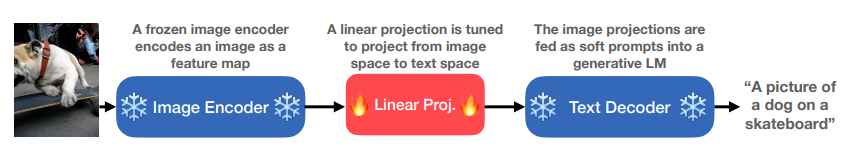
\includegraphics[width=\linewidth]{images/fig3.PNG}
	\caption{
		The architecture of LimBeR. Linear projection map image representations into input space of language model. this linear projection enable to produce captions describing images.}
	\vspace{-2mm}
        \label{fig:limberarch}
\end{figure}

\newpage
\bibliography{egbib}

\end{document}
